%%%%%%%%%%%%%%%%%%%%%%%%%%%%%%%%%%%%%%%%%%%%%%%%%%%%%%%%%%%%%%%%%%%%%%%%%%%%%%%%
%2345678901234567890123456789012345678901234567890123456789012345678901234567890
%        1         2         3         4         5         6         7         8

\documentclass[letterpaper, 10 pt, conference]{ieeeconf}  % Comment this line out
                                                          % if you need a4paper
%\documentclass[a4paper, 10pt, conference]{ieeeconf}      % Use this line for a4
                                                          % paper

\IEEEoverridecommandlockouts                              % This command is only
                                                          % needed if you want to
                                                          % use the \thanks command
                                                          \usepackage[utf8]{inputenc}
\usepackage[utf8]{inputenc}
\overrideIEEEmargins
% See the \addtolength command later in the file to balance the column lengths
% on the last page of the document



% The following packages can be found on http:\\www.ctan.org
%\usepackage{graphics} % for pdf, bitmapped graphics files
%\usepackage{epsfig} % for postscript graphics files
%\usepackage{mathptmx} % assumes new font selection scheme installed
%\usepackage{times} % assumes new font selection scheme installed
\usepackage{amsmath} % assumes amsmath package installed
\usepackage{amssymb}  % assumes amsmath package installed
\usepackage{fancyhdr}
\setlength{\headheight}{15.2pt}
\usepackage[]{algorithm2e}
\usepackage{url}
\usepackage{graphicx}

\newtheorem{thm}{Theorem}
\newtheorem{lem}{Lemma}
\newtheorem{defi}{Definition}
\newtheorem{prop}{Proposition}
\usepackage{listings}

\title{\LARGE \bf
%modif
On the vulnerabilities of the DHCP protocol
}

\author{Benjámin Martin Seregi$^{1}$% <-this % stops a space
% \thanks{*This work was not supported by any organization}% <-this % stops a space
\thanks{$^{1}$ e-mail: seregi@kth.se}%
}

\begin{document}


\maketitle
\thispagestyle{fancy}
\fancyhf{}
\chead{KTH Royal Institute of Technology | EP2510, Fall 2017, Period 2 | \today}

\begin{abstract}
The Dynamic Host Configuration Protocol (DHCP) is a widely used protocol for dynamically distributing Internet (IP) addresses. The protocol is also responsible for the dynamic distribution of the DNS server and gateway addresses. Due its unauthenticated communication, man-in-the-middle attacks can be carried out by rogue DHCP servers providing malicious DNS or gateway addresses. In this report we investigate the state-of-the-art techniques that mitigate DHCP attacks and we propose a new extension of the DHCP protocol that protects against rogue DHCP servers. In addition, we implement this extension using the INET Framework and run simulations in OMNeT++.
\end{abstract}

\begin{keywords}
DHCP, rogue DHCP server, DHCP authentication, DHCP spoofing, DHCP security
\end{keywords}
% TODO: dhcp snooping, dhcp authentication: with public key crypthography,
% wlc, description of the different attacks
% unicast / broadcast client-server communication (broadcast flag in DHCP)
% https://www.cisco.com/c/en/us/td/docs/solutions/Enterprise/Mobility/emob41dg/emob41dg-wrapper/ch4_Secu.html#wp1019184

%%%%%%%%%%%%%%%%%%%%%%%%%%%%%%%%%%%%%%%%%%%%%%%%%%%%%%%%%%%%%%%%%%%%%%%%%%%%%%%%
\section{Introduction}
%Describe the background for chosen area that is going to be investigated. Write a short description of the area that is going to be %investigated. It is a brief description of the necessary background knowledge of the problem area and for carrying out the project.
The Dynamic Host Configuration Protocol is a widely used protocol for dynamically distributing Internet addresses \cite{dhcprfc}. DHCP works in a client-server architecture where the client (DHCP client) requests an IP address and the server (DHCP server) allocates IPs from the pool of available addresses. The communication between these two entities is unauthenticated \cite{dhcprfc} which imposes several security issues. Rogue DHCP server can be easily set up that might offer the clients malicious default gateways or DNS servers (see \cite{dhcprfc}, DHCPOFFER message) that can lead to denial-of-service or man-in-the-middle attacks \cite{Rooney:2010:IIA:1951974} (9 Security Considerations). In addition, the lack of authentication allows the attacker to exhaust the pool of available addresses by continuously requesting new IPs using fake MAC addresses and request DHCP operations (e.g. DHCP lease) on behalf of other clients by fabricating DHCP messages with sniffed MAC addresses (hijacking) \cite{practical-embedded-security} (Chapter 2).

In this report we overview the state-of-the-art countermeasures against DHCP attacks. We also introduce a new extension of the DHCP protocol that prevents man-in-the-middle attacks. In addition, we implement this extension using the open-source INET Framework \cite{inet} and run simulations in OMNeT++ \cite{Varga:2008:OOS:1416222.1416290}. The aim of the simulations is to show how DHCP vulnerabilities can lead to man-in-the-middle attacks and to demonstrate that this new extension can prevent them. The rest of the report is organized as follows.

Section \ref{sec:man-in-the-middle} describes a possible man-in-the-middle attack when we use the base protocol, that is, the RFC 2131 without any additional modifications. In Section \ref{sec:dhcp-snooping}, we discuss the DHCP snooping technique which is a L2 security tool against DHCP hijacking and rogue DHCP servers. 

In Section \ref{sec:auth}, we investigate the different DHCP authentication techniques with a high focus on public key cryptography.

In Section \ref{sec:protected-mode}, we introduce a possible extension of the existing DHCP implementation that protects against rogue DHCP servers. The main advantage of our extension that it does not require any pre-configuration unlike the different DHCP authentication extensions but it performs a verification where each DHCPREQUEST should be approved by all DHCP servers in the network. This makes it possible using this extension where the pre-configuration of the user's device is impossible such as in a WiFi hotspot.
 
\section{A man-in-the-middle attack with a rogue DHCP server}\label{sec:man-in-the-middle}
Man-in-the middle attacks happen when the communication between the network devices is intercepted by an untrusted entity (e.g. DNS server, default gateway). Although they provide the same services as their trusted counterparts to deceive the users, they can alter (e.g. DNS server) and eavesdrop on (e.g. default gateway) the communication.

In what follows I would like demonstrate a possible man-in-the-middle attack carried out by an untrusted default gateway with the a help of a rogue DHCP server. Let us assume that the user connects to a regular IEEE 802.11 access point in a restaurant. The main steps of the attack are as follows:
\begin{enumerate}
\item Once the user's device is connected to the access point (L2 connection), the DHCP client initiates the IP address allocation process by broadcasting a DHCPDISCOVER message (\cite{dhcprfc} 3.1 Client-server interaction - allocating a network address, 1.). Assume that the attacker has implemented a rogue DHCP server that acts like a usual DHCP server, the only exception that it provides untrusted default gateway address. This untrusted gateway implemented by the attacker provides Internet access to deceive the user. The user will not be suspicious as he will have stable Internet access, however, the attacker can eavesdrop on the outgoing user data-flow at the untrusted default gateway.
\item When the DHCPDISCOVER arrives at the DHCP servers, they may reply with a DHCPOFFER message (\cite{dhcprfc} 3.1 Client-server interaction - allocating a network address, 2.). In the DHCPOFFER packet each server offers an available IP address and includes gateway and DNS addresses in the packet's options field. Let us assume that the rogue DHCP server offers an untrusted gateway address to the user. This untrusted gateway provides Internet access and it is eavesdropping on the user communication gaining access to sensitive data such as passwords.
\item Let us assume that the rogue DHCP sever is faster in the sense that its DHCPOFFER arrives faster than the trusted one. RFC 2131 does not define what to do when there are multiple responses, the user can wait for more responses or can accept the first offer (\cite{dhcprfc} 3.1 Client-server interaction - allocating a network address, 3.). Let us assume that the DHCP client accepts the first reply. In this case, the user broadcasts a DHCPREQUEST packet with the configuration information provided in the offer. After that the rogue DHCP server acknowledges the request by sending a DHCPACK (\cite{dhcprfc} 3.1 Client-server interaction - allocating a network address, 4.).
\item Finally, the clients start communicating using the untrusted default gateway.
\end{enumerate}
From the above example we can see that it is very easy to carry out man-in-the-middle attacks with the help of rogue DHCP servers. The main problem is that the user cannot decide whether the received DHCP configuration parameters are valid or not. If the user's DHCP client had known that the DHCP packets were coming from an untrusted server, it could drop them immediately providing security to the user.
\section{DHCP Snooping}\label{sec:dhcp-snooping}
\section{DHCP authentication methods}\label{sec:auth}

TODO: \cite{7208238} and \cite{6866756}

\section{A new extension: DHCP Protected Mode}\label{sec:protected-mode}
DHCP protected mode is an extension of the existing (RFC 2131) DHCP protocol. The basic idea is that every DHCP server verifies each DHCPREQUEST packet with a DHCPACK and can signal a warning with a DHCPNAK if the DHCPREQUEST packet contains some untrusted information such as unknown DNS or default gateway addresses that are not in the list of trusted addresses of the DCHP server. The fact that each DHCPREQUEST packet is being sent to the broadcast address gives the opportunity to each DHCP server to examine its content and therefore it can alert the DHCP client to a possible attack by sending a DHCPNAK.

This extension has been implemented in the INET Framework as an optional feature in DHCP. The source code is open-source and available at \url{https://github.com/Benmartin92/netsec-kth}.

To experiment with the implementation we have built a simulation scenario (see Fig. \ref{fig:topology}) that consists of a \textit{client} who requests an IP address and two DHCP servers; one of them (\textit{rogueDHCPServer)} attempts to provide untrusted default gateway address (\textit{rogueGateway}) where the outgoing user data is being eavesdropped on by the attacker. The simulation files can be found at \texttt{inet/examples/anssdhcp} in the GitHub repository. In Section \ref{sec:man-in-the-middle} 3), we assumed that the rogue DHCP server is faster, that is, its responses arrive first at the client. We simulate this assumption by implementing a faster link between the access point (\textit{ap}) and \textit{rougeDHCPServer} as you can see from the following code snippet (for more details, see \texttt{ANSSManInTheMiddle.ned}.
\begin{verbatim}
network ANSSManInTheMiddle
{
	...
    connections:
        gateway.pppg++ <--> 
        Eth100M <--> Internet.pppg++;
        gateway.ethg++ <--> 
        Eth100M <--> ap.ethg++;
        rogueGateway.pppg++ <--> 
        Eth100M <--> Internet.pppg++;
        remoteServer.pppg++ <--> 
        Eth100M <--> Internet.pppg++;
        dhcpServer.ethg++ <--> 
        Eth100M <--> ap.ethg++;
        rogueDHCPServer.ethg++ <--> 
        Eth1G <--> ap.ethg++;
        rogueGateway.ethg++ <--> 
        Eth100M <--> ap.ethg++;
}
\end{verbatim}
When the DHCPOFFER arrives at the \textit{client} and protected mode is off, it accepts the offer immediately by sending a DHCPREQUEST with the received configuration parameters and starts communication via \textit{rogueGateway}.

However, if we turn on the protected mode, the DHCPREQUEST sent by \textit{client} will be investigated by \textit{dhcpServer} which has the list of trusted gateway addresses. Even though \textit{rougeDHCPServer} acknowledges the request by sending a DHCPACK, \textit{client} will not start using the network (in contrary to \cite{dhcprfc} 3.1 Client-server interaction - allocating a network address, 5.) until its \texttt{protectionInterval} times out. This time window that can be configured by the network administrator gives the chance to the trusted servers to send a DHCPNAK if the gateway address is not in their whitelist. If the DHCP client receives at least one DHCPNAK within this interval, it will not start communicating with the default gateway but it will notify the user and restart the DHCP process by sending a DHCPDISCOVER.

Advantages (TODO):
\begin{itemize}
\item cheap (no expensive and fancy cisco hardwares needed)
\item no preconfiguration needed at client side
\item computationally inexpensive (authentication can be expensive)
\item easy to implement
\end{itemize}

The drawbacks of this extension (TODO):
\begin{itemize}
\item additional time because of the protection interval - but this is negligible
\item requires protocol state machine modifications both client and server side (but NO new packets needed)
\item the rogueDHCP server can repeat the whole process arbitrary times. repeating the whole process would result in no connection at all,
but it is still better than being eavesdropped on.
\item rogue DHCP server can DHCPNAK valid gateway addresses, but again this is still better than being eavesdropped on.
\end{itemize}
\addtolength{\textheight}{-12cm}   % This command serves to balance the column lengths
                                  % on the last page of the document manually. It shortens
                                  % the textheight of the last page by a suitable amount.
                                  % This command does not take effect until the next page
                                  % so it should come on the page before the last. Make
                                  % sure that you do not shorten the textheight too much.

%%%%%%%%%%%%%%%%%%%%%%%%%%%%%%%%%%%%%%%%%%%%%%%%%%%%%%%%%%%%%%%%%%%%%%%

\bibliographystyle{IEEEtran}
\bibliography{ref.bib}
\begin{figure*}
\centering
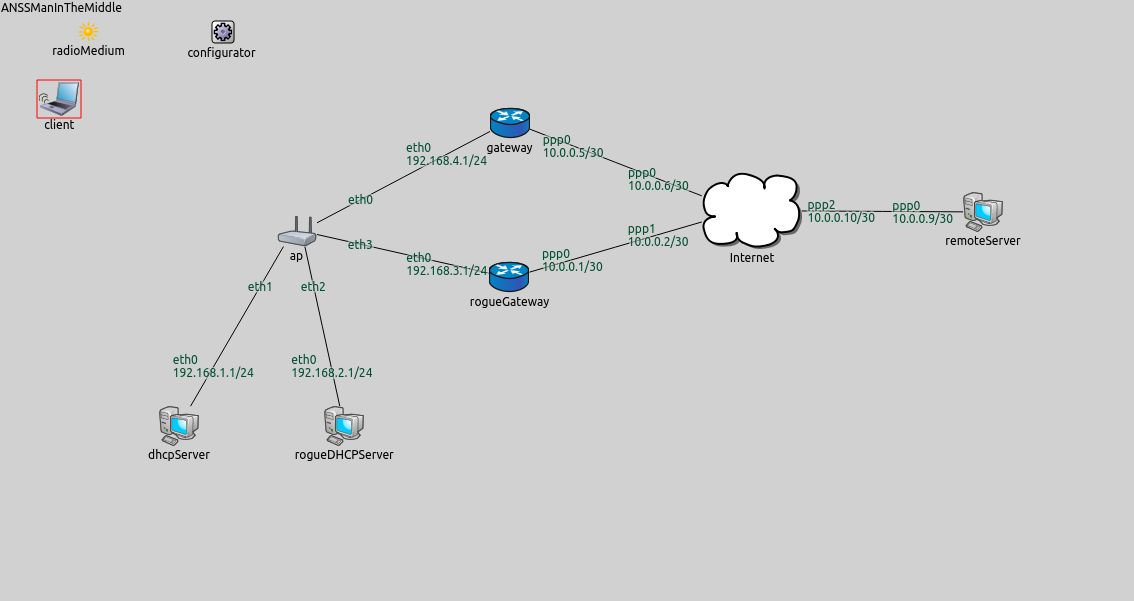
\includegraphics[scale=0.4]{figures/topology.png}
\caption{Man-in-the-middle attack simulation topology with a rogue DHCP server}\label{fig:topology}
\end{figure*}
\end{document}